\section{Performance}

The response of the LTCC to electrons and pions has been studied using experimental data from the spring 2019
run period, the first time that the LTCC s3 and s5 boxes were filled with C$_4$F$_{10}$ gas. At the time of this
writing the data is not yet fully calibrated. However the CLAS12 detectors are sufficiently well calibrated to
understand several fundamentals aspects of the LTCC response.

\subsection{LTCC Response to Electrons}
\label{sec:elecResponse}

The electrons are selected using the reconstruction algorithms~\cite{recon-nim} that identify electron tracks. The
LTCC response is calculated by checking whether the electrons produced a signal in the detector or not. The electron
momenta has been selected in the expected pion response range, between 3.5 and 8~GeV. The criteria for event
selection are:

\begin{itemize}
\item  Electrons identified using the reconstruction Event Builder algorithm;
\item Electrons must be within the geometrical fiducial volume of the LTCC.
\end{itemize}


The electron momentum spectrum before and after the requirement of an associated LTCC signal is shown in
\F{electronEfficiency}, along with a 0$^{th}$-order polynomial fit. The average efficiency for detection of
electrons in the LTCC is 94$\%$, slightly below the expected efficiency of 99$\%$. This may be due to
several reasons:

\begin{itemize}
\item the electron selection was not refined by using the calorimeters (due to the uncalibrated detector status);
\item possible impurities in the gas, which was not purified by the recovery system (unavailable at that time);
\item the data analyzed were not fully calibrated at the time of this writing;
\item the mirror overlaps and re-positioning issues mentioned in Section~\ref{sec:possibleInefficiency}.
\end{itemize}

\begin{figure}[ht]
	\centering
	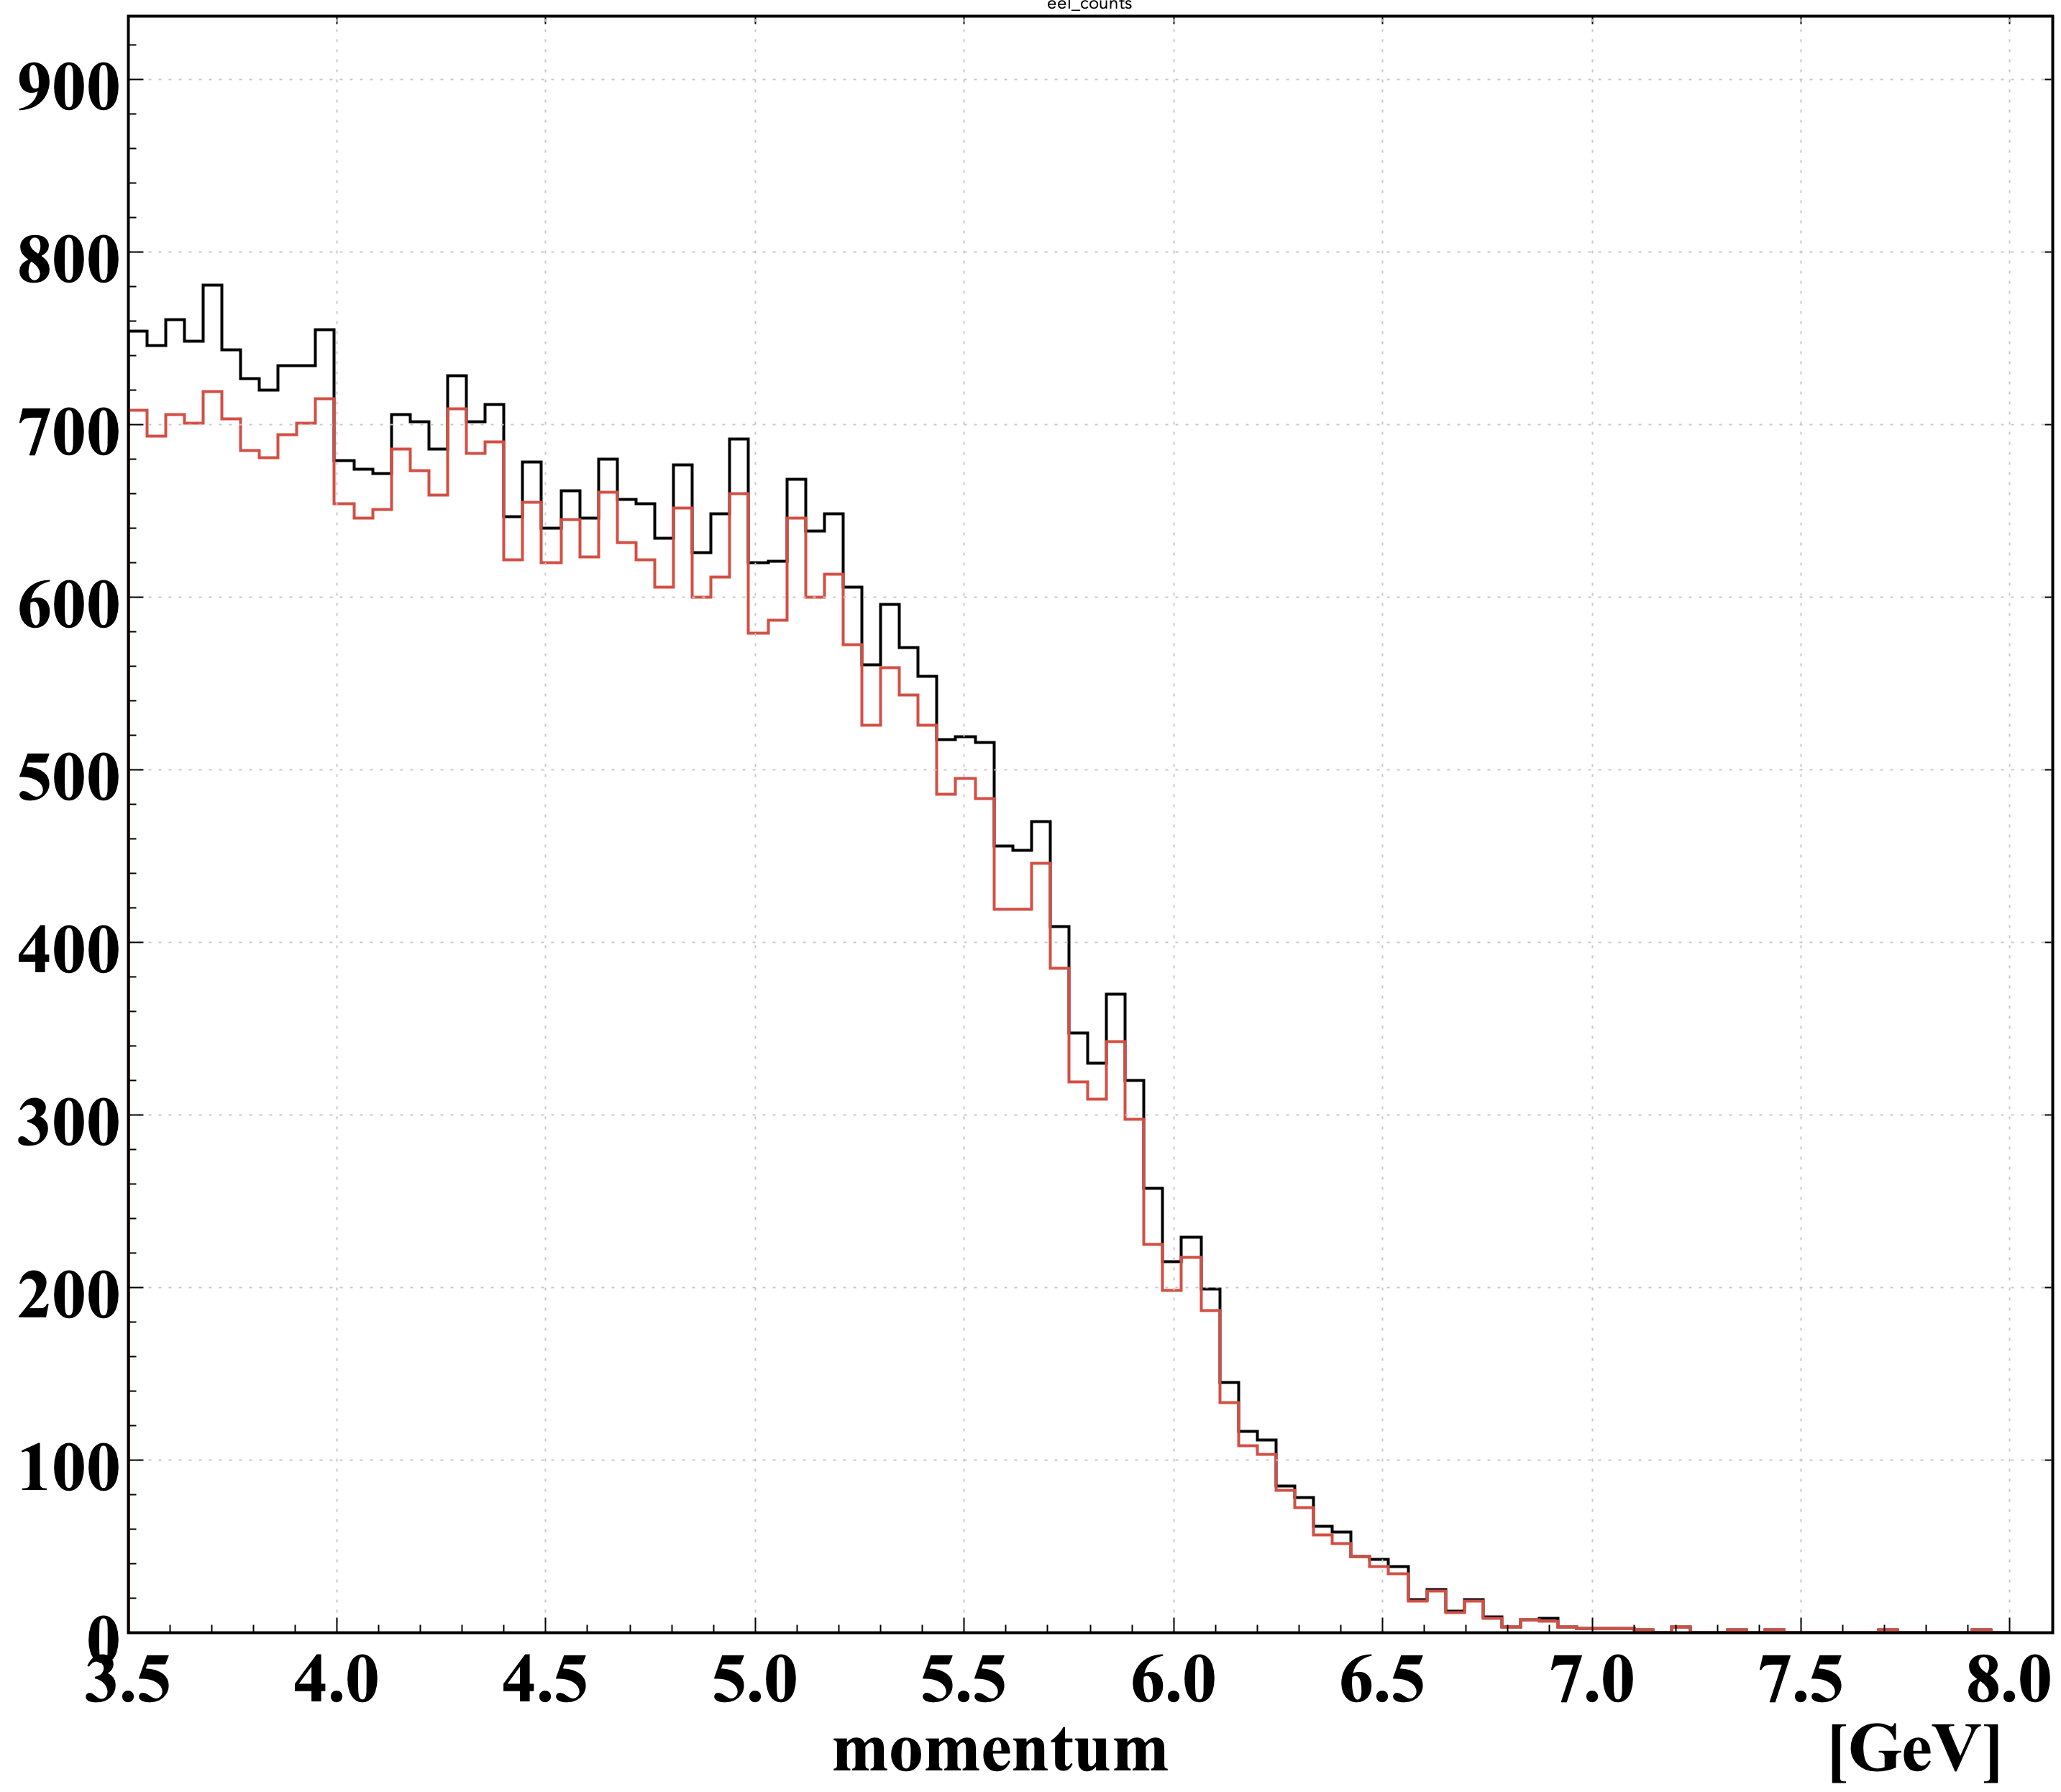
\includegraphics[width=0.98\columnwidth,keepaspectratio]{img/electronMomenta.png}
	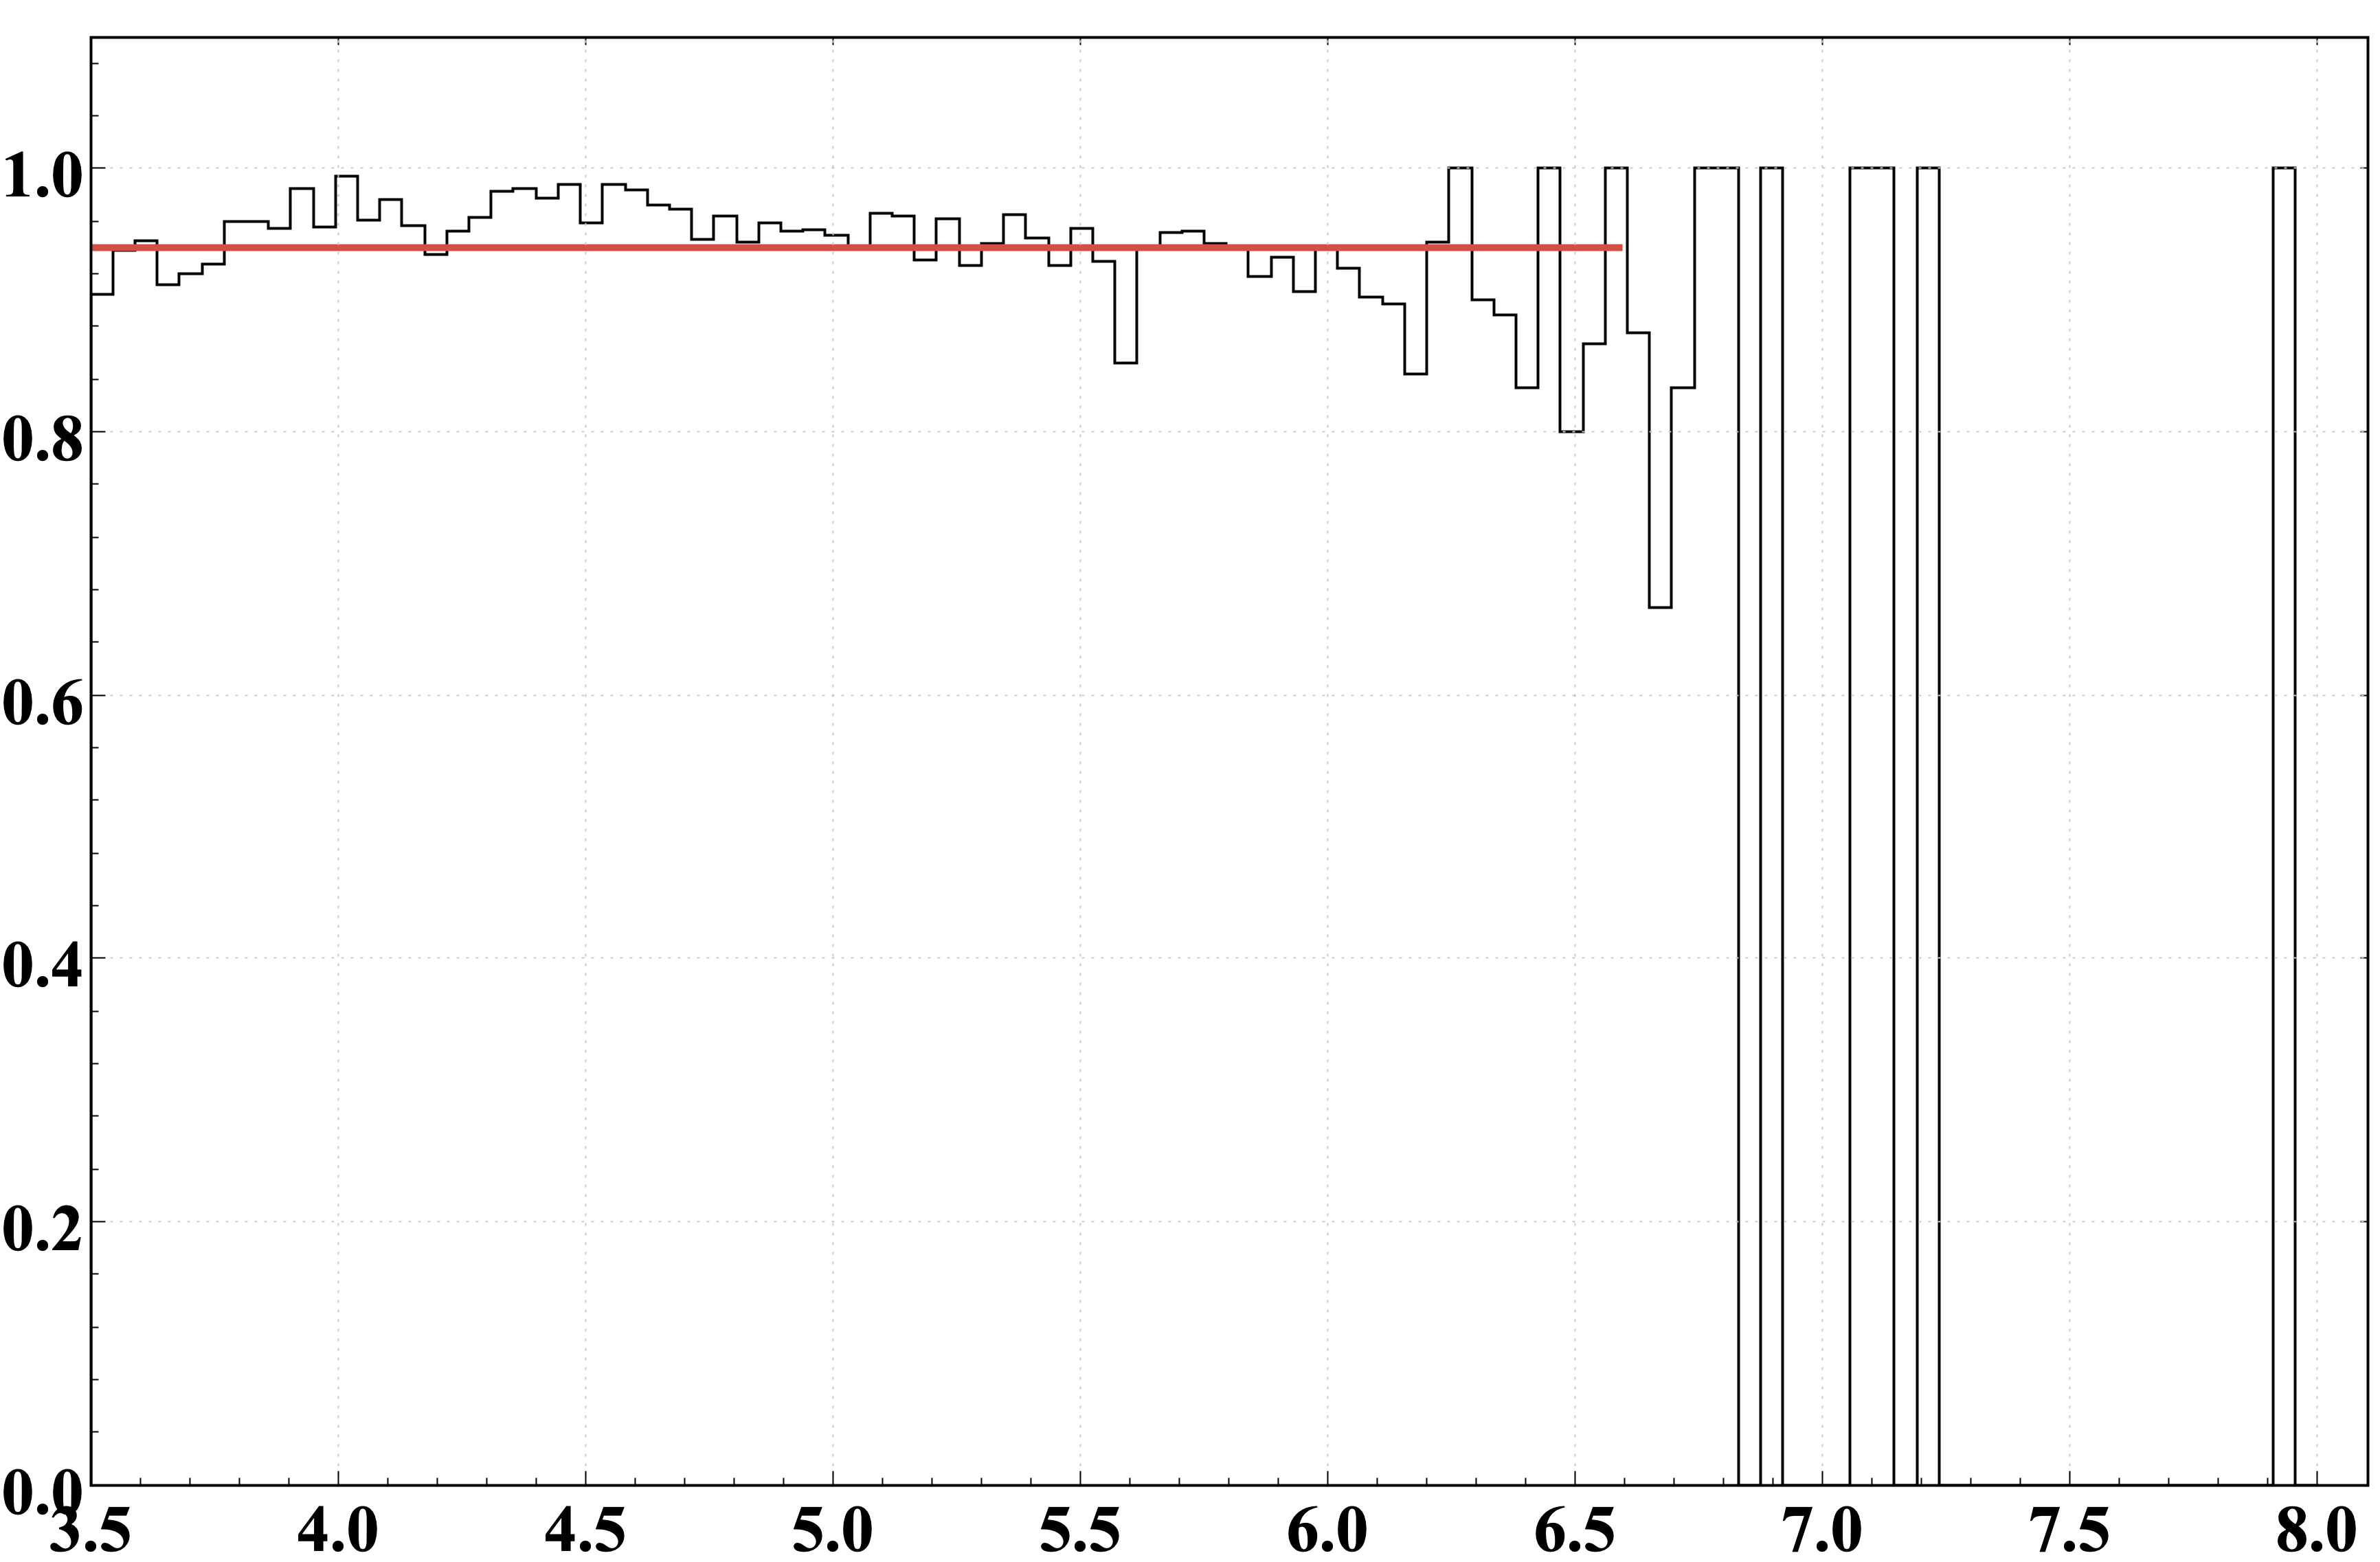
\includegraphics[width=0.98\columnwidth,keepaspectratio]{img/electronEfficiency.png}
	\caption{Top: the number of reconstructed electrons vs. momentum (GeV) before and after the requirement of
          an associated LTCC signal. Bottom: the LTCC efficiency to electrons is the ratio of the two distributions above.
          A 0$^{th}$-order polynomial fit gives an average of 94$\%$ efficiency.}
	\label{fig:electronEfficiency}
\end{figure}

\subsection{LTCC Response to Pions}

The determine the response of the LTCC to pions, reconstructed positively charged pions were selected and a check
was done on whether they produced a good signal in the LTCC detector. The positive pion selection considers all
positively charged particles that pass a neutron missing mass cut for the reaction $ep \to e'\pi^+n$. The criteria
for event selection are:

\begin{itemize}
    \item The electron selection described in Section~\ref{sec:elecResponse};
    \item Positive pion candidates are identified using the reconstruction Event Builder algorithm;
    \item The positive pion candidates must be within the LTCC geometrical fiducial volume;
    \item A neutron missing mass cut is applied between 0.9 and 1.05~GeV (see \F{neutronMM}).
\end{itemize}

The missing mass cut is shown in \F{neutronMM}. The positive pion candidates that satisfy the cuts are shown in black
and those with a good LTCC cluster associated with the track are shown in red.

\begin{figure}[H]
	\centering
	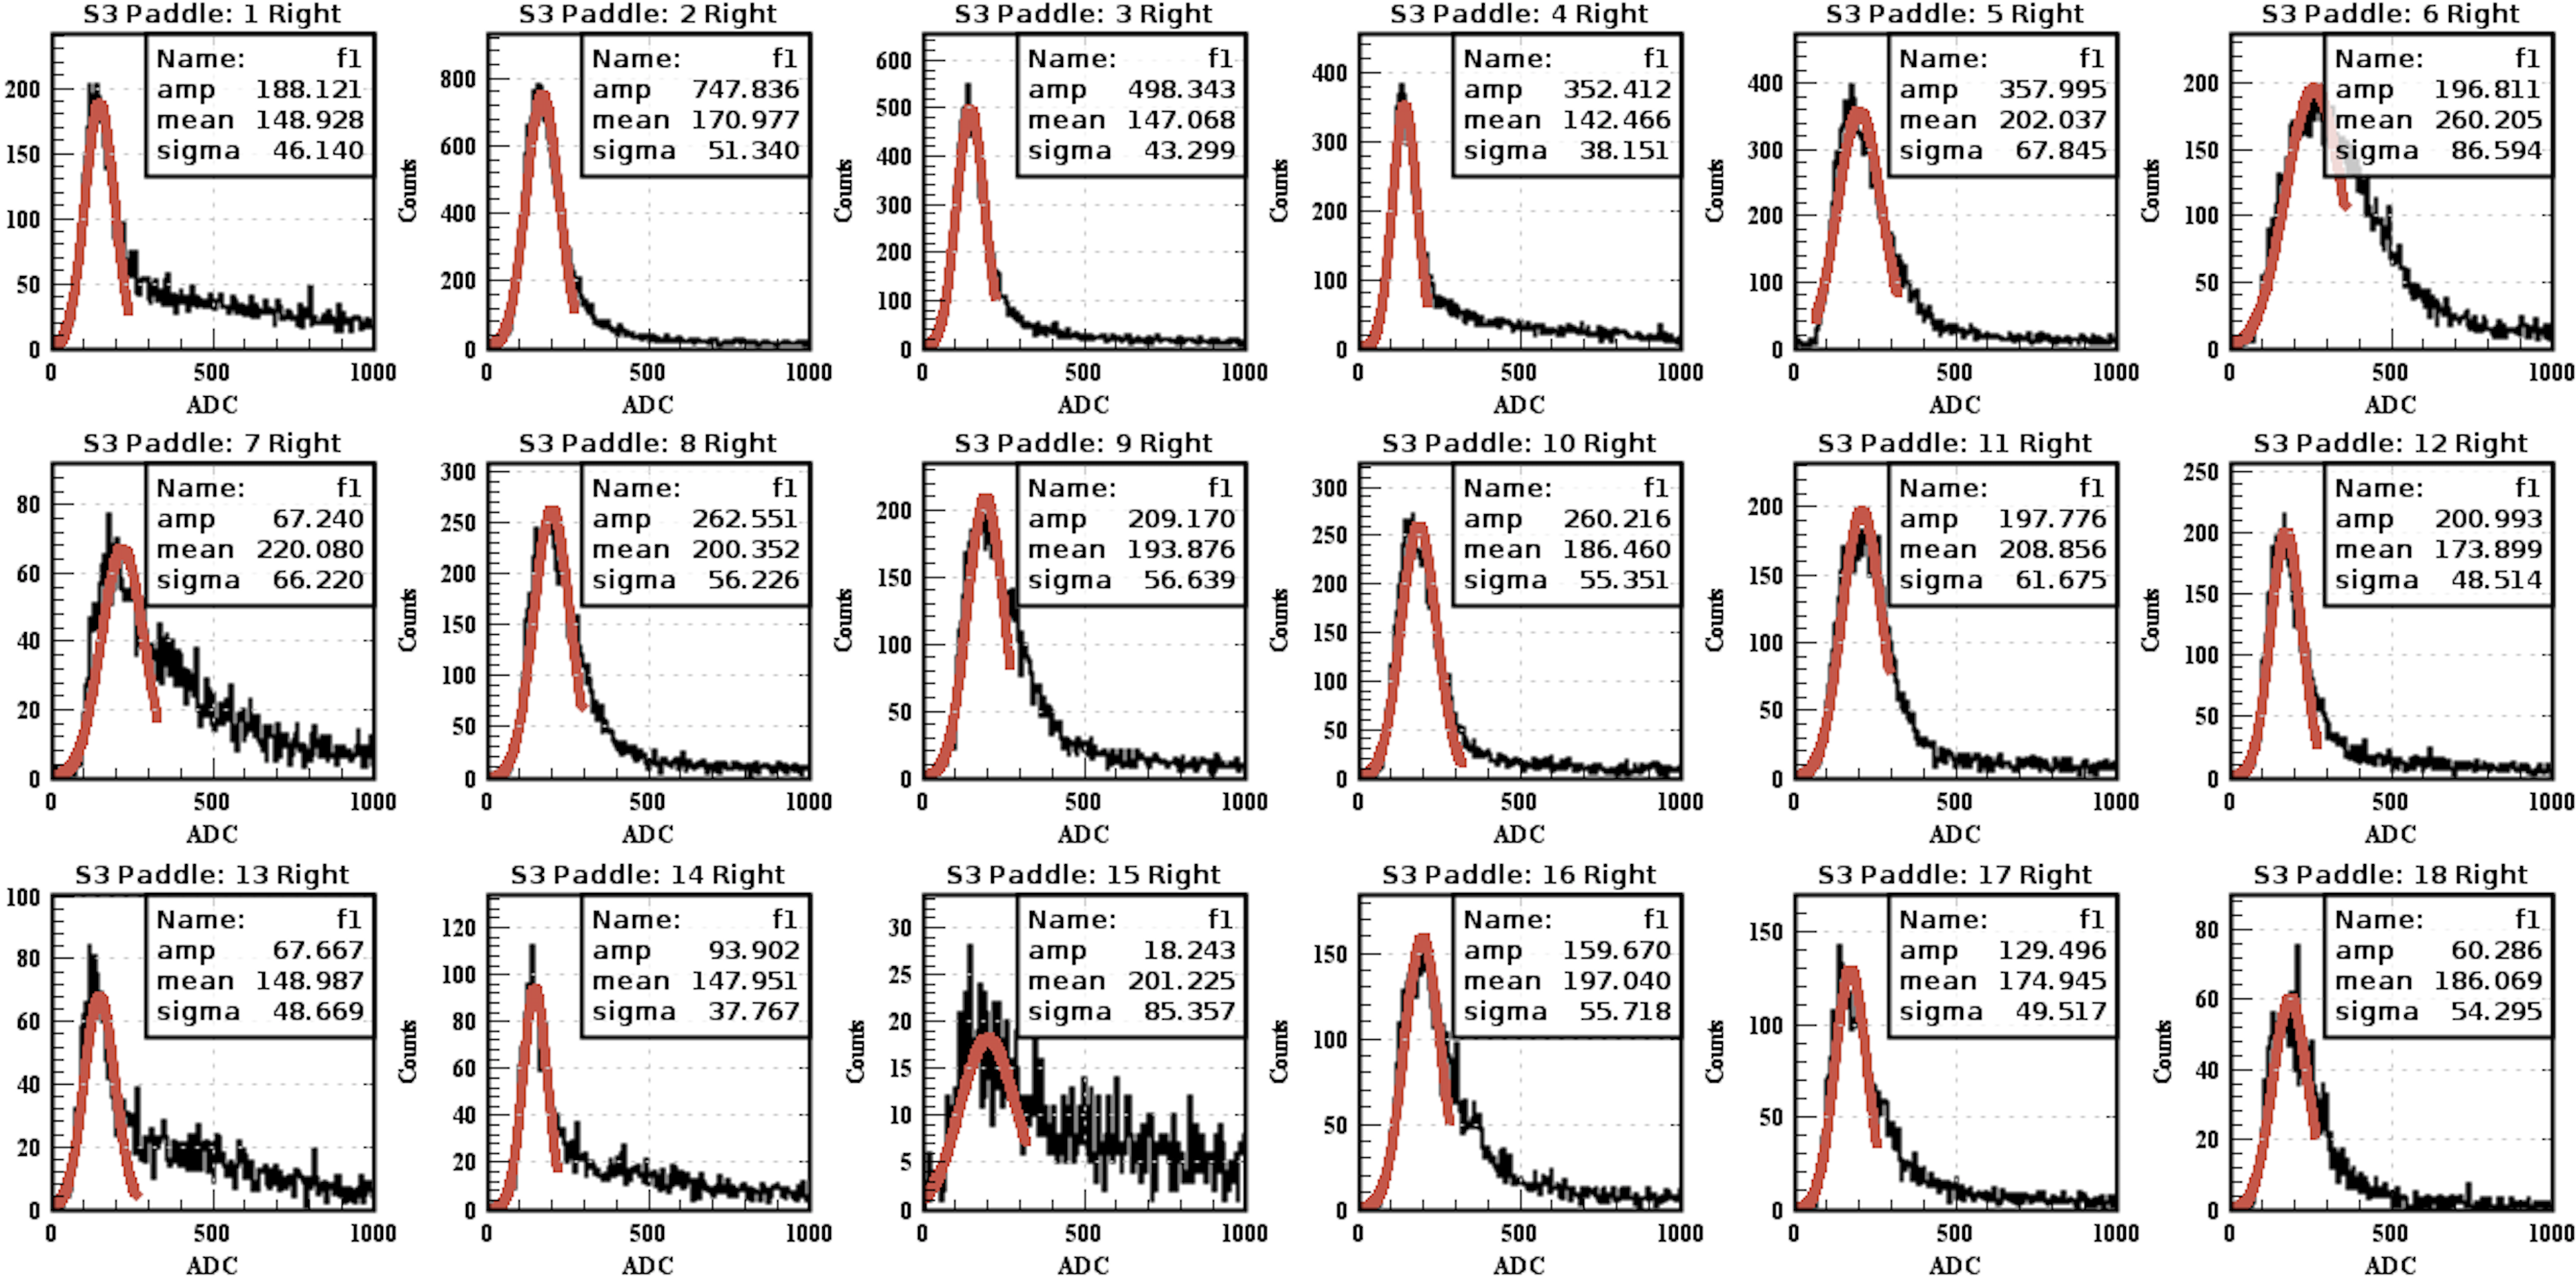
\includegraphics[width=0.98\columnwidth,keepaspectratio]{img/neutronMM.png}
	\caption{The missing mass from the reaction $ep \to e'\pi^+X$, where the peak at the neutron mass
          between 0.95 and 1.05~GeV is selected for the efficiency analysis. The positive pion candidates that
          satisfy the cuts are shown in black. The pions associated with an LTCC signal are shown in red.}
	\label{fig:neutronMM}
\end{figure}

\begin{figure}[H]
	\centering
	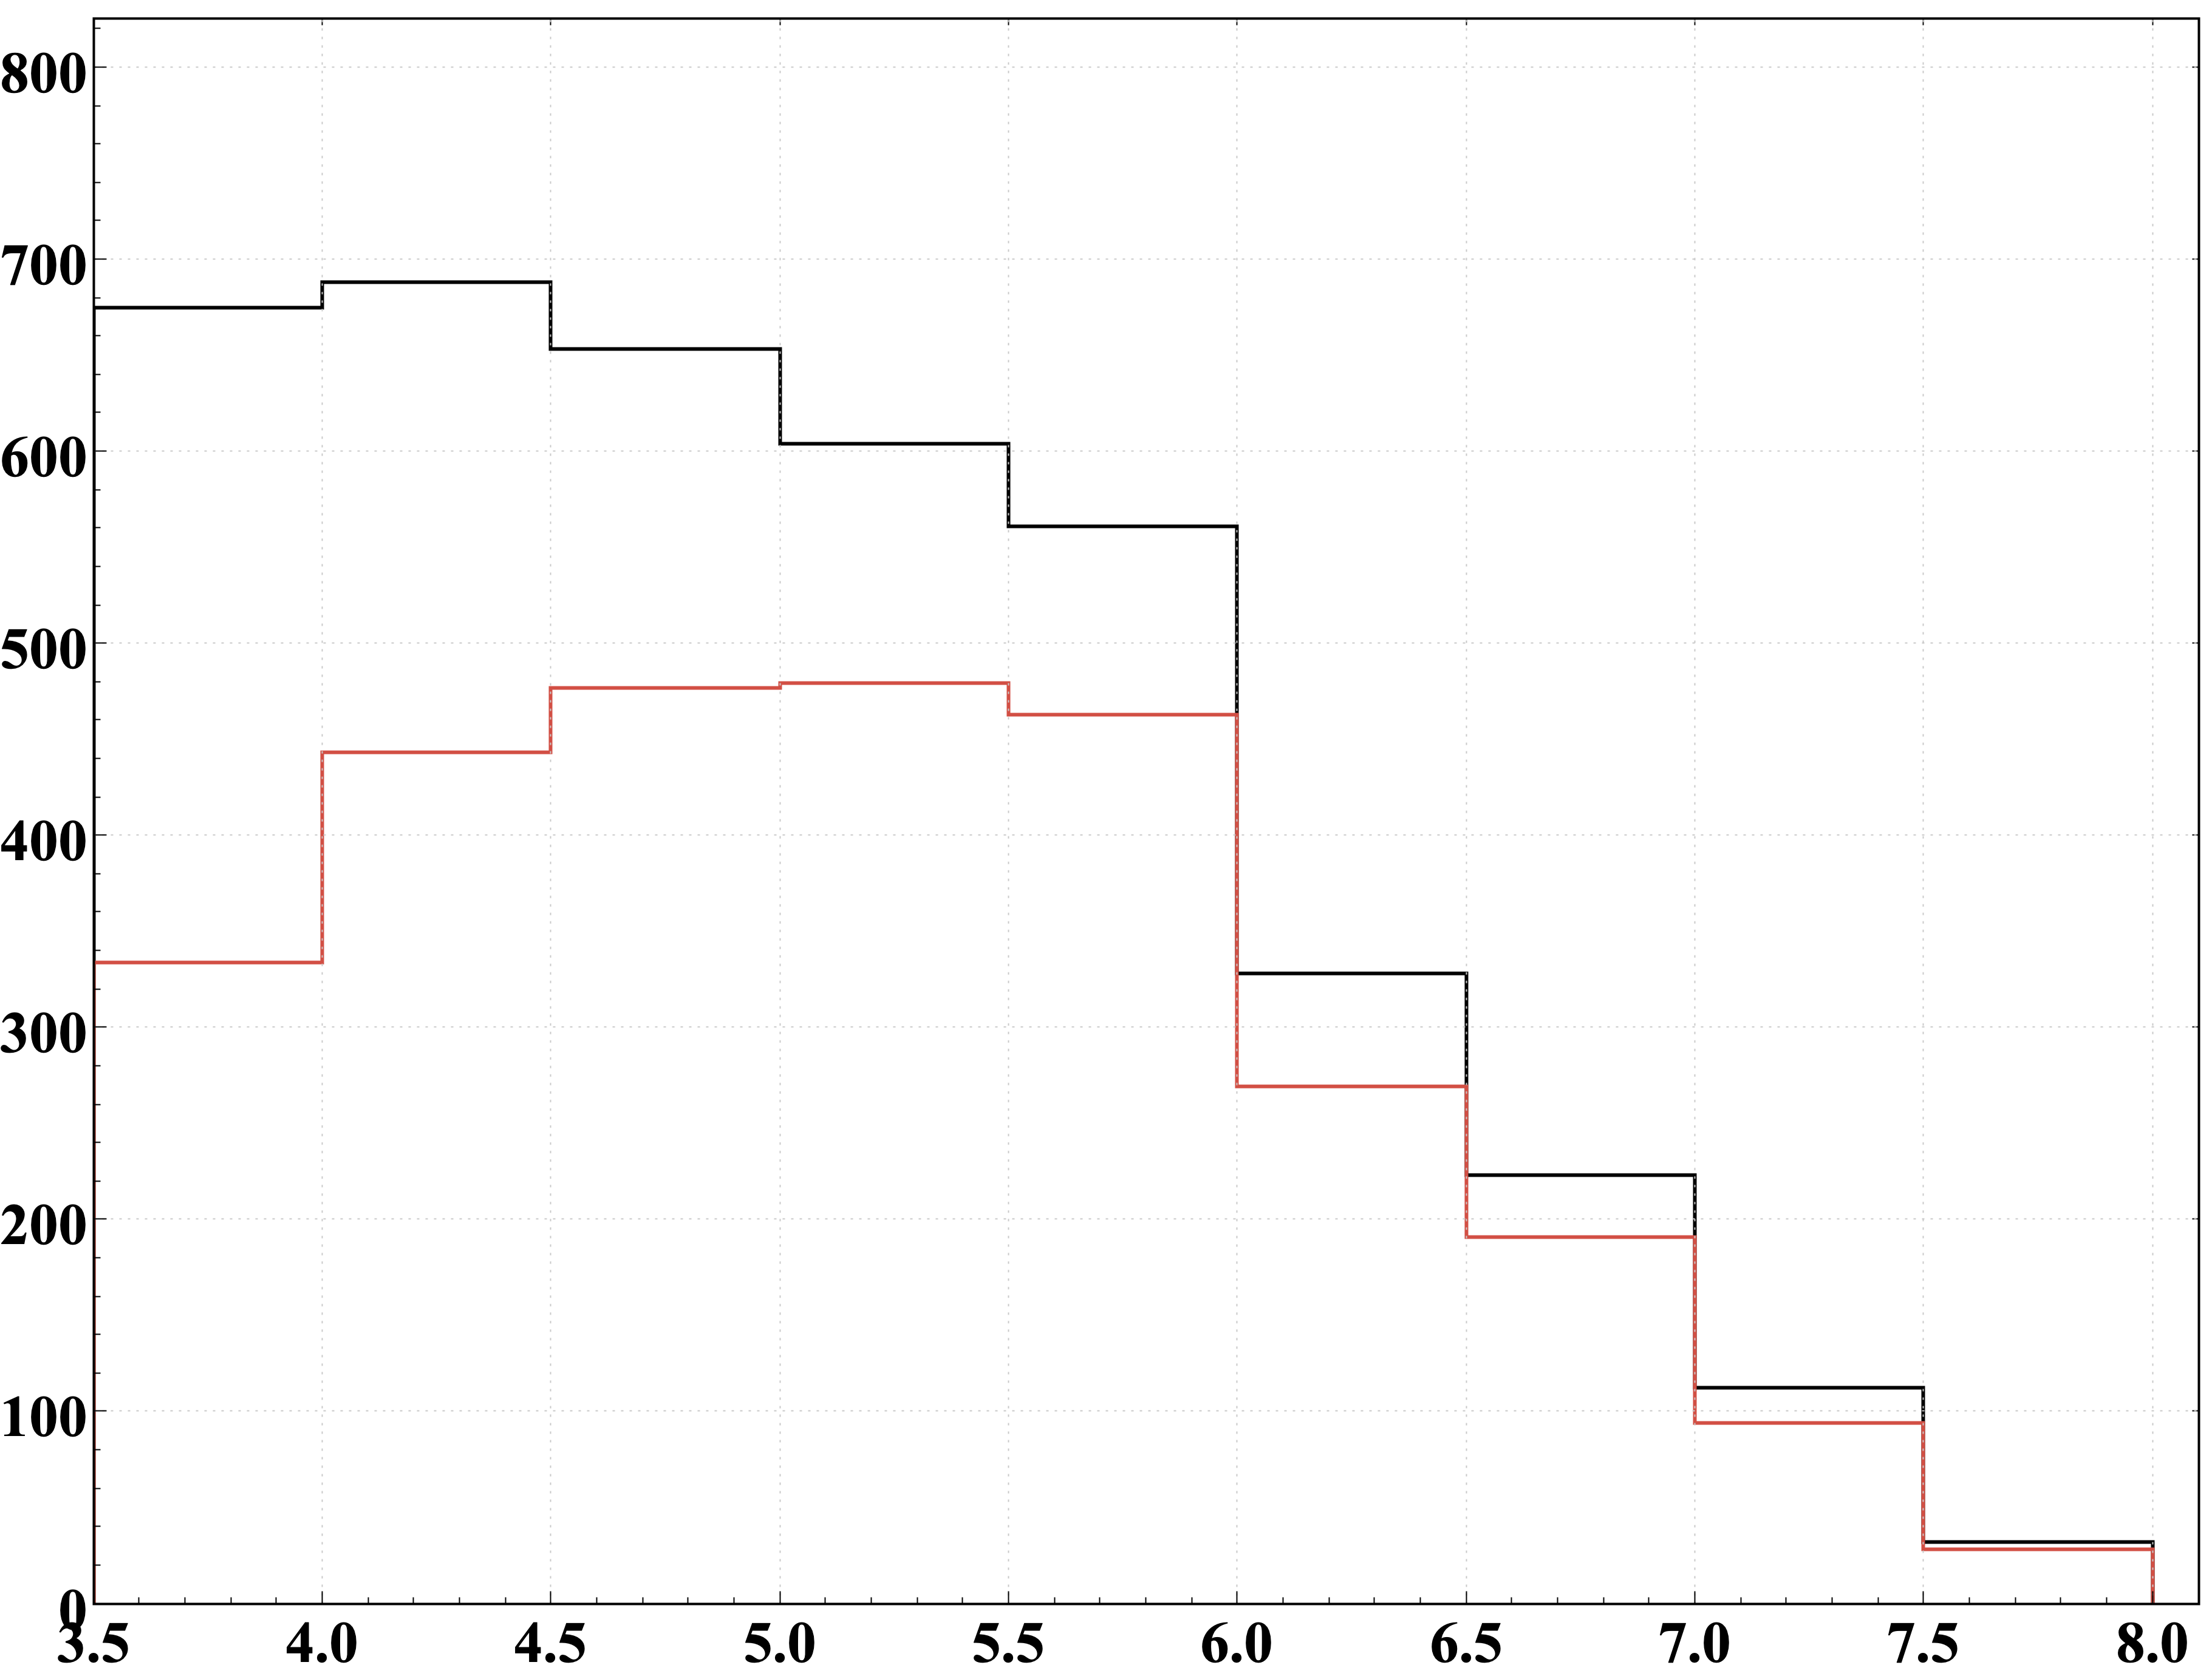
\includegraphics[width=0.98\columnwidth, height=0.7\columnwidth]{img/pionMomentum.png}
	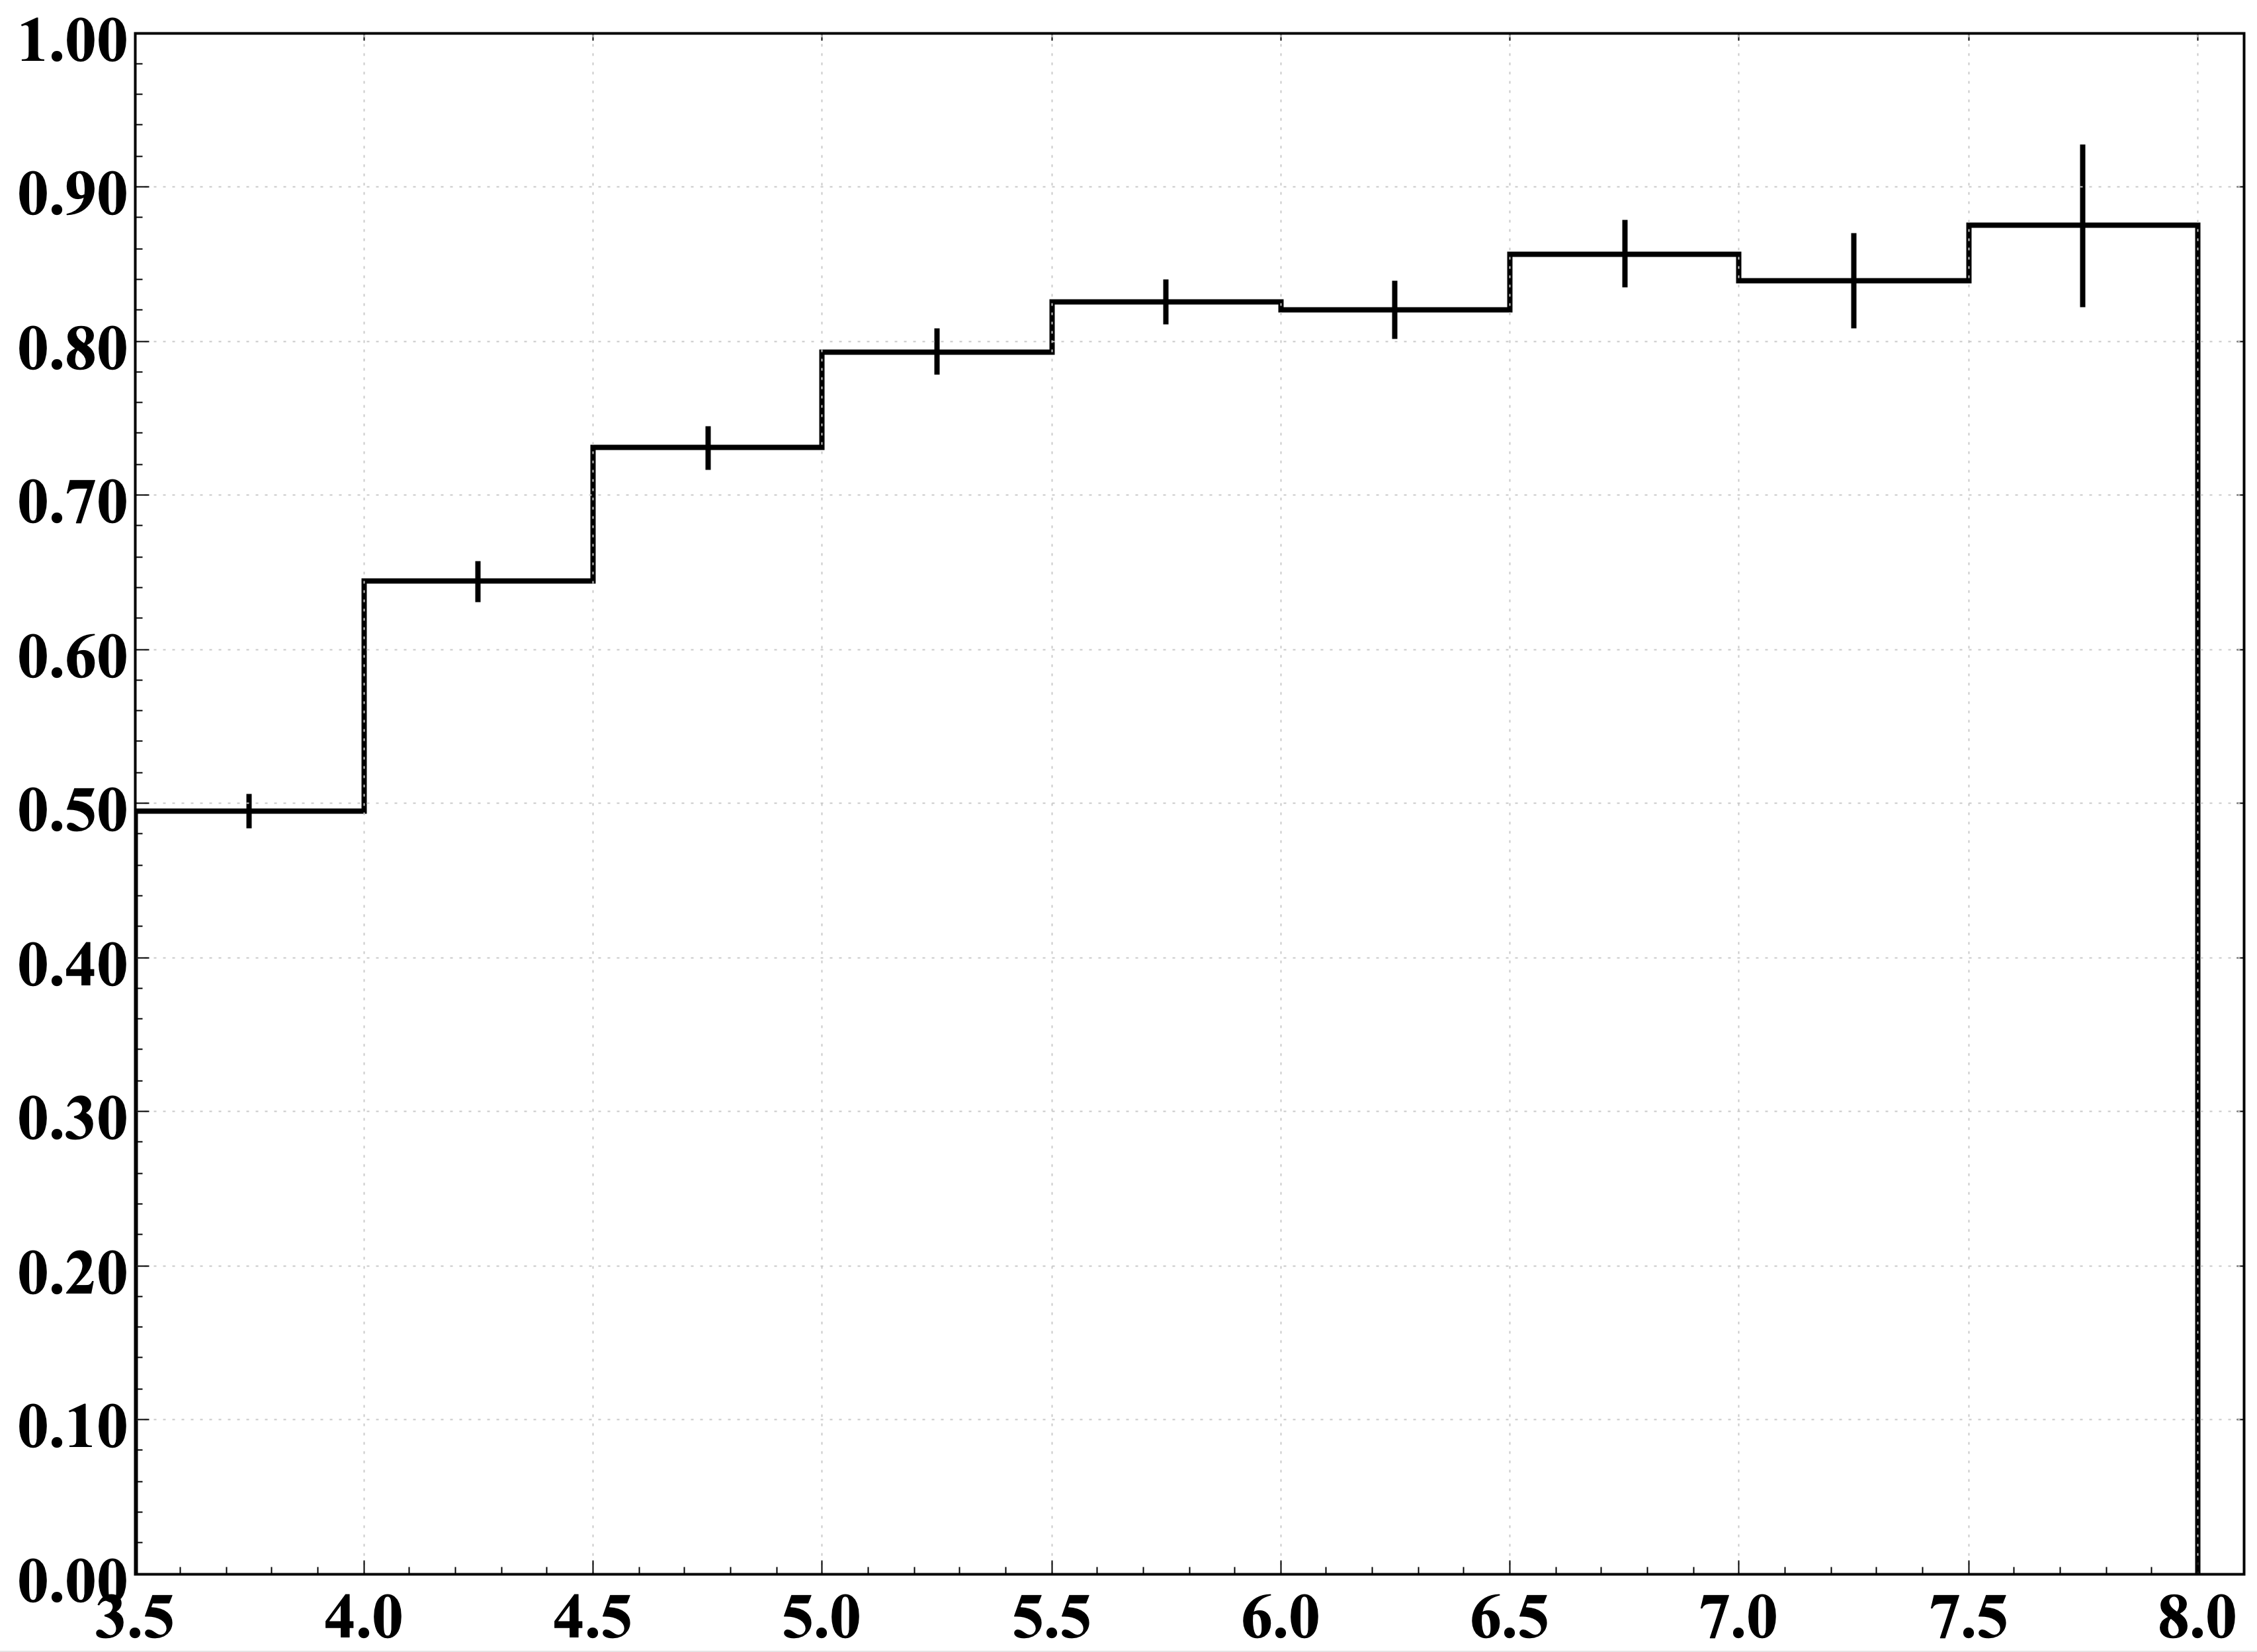
\includegraphics[width=0.98\columnwidth, height=0.7\columnwidth]{img/pionEfficiency.png}
	\caption{Top: The pion momentum distribution before and after the requirement of an associated LTCC signal.
          Bottom: The LTCC pion efficiency as a function of momentum. This is the ratio of the curves shown on top
          normalized by the average electron efficiency of 94\% shown in \F{electronEfficiency}.}
	\label{fig:pionMomentum}
\end{figure}

The momentum distribution of the pions is shown in \F{pionMomentum} (top) for all pions and for the pions with an
associated signal in the LTCC. The ratio, normalized by the electron efficiency of 94\% found above to account for
other system inefficiencies, defines the LTCC pion detection efficiency as a function of momentum (see
Fig.~\ref{fig:pionMomentum} bottom). The LTCC response starts around 50\% near the expected signal threshold of
$\sim$3.5~GeV, and rises with momentum as expected, given that the number of emitted photons increases with
momentum. A plateau of 88\% is reached after a momentum of 5~GeV. This is within range of an expectation of
the expected efficiency above 90\%.
